%!TEX program = xelatex
\documentclass{article}
\usepackage{ctex}
\usepackage{amsmath,amssymb}
\usepackage{graphicx}

\begin{document}
	\begin{abstract}
		本次作业用\LaTeX 写。
	\end{abstract}
\begin{itemize}
	\item[1.] 证明:曲线$c(t) = \left(\dfrac{1 + t^2}{t} , t+1, \dfrac{1-t}{t}\right)$是平面曲线。
	
	证明: 因为$x(t) = \dfrac{1}{t} + t, y(t) = t+1, z(t) = \dfrac{1}{t}-1$ \\
	所以$x(t) = y(t) + z(t).$所以在平面$x = y + z$上。\\
	(也可用绕率为0)
	\item[2.] 画出轨迹图, 计算外摆线参数
	
	
	解: 设两个圆分别旋转了$\theta_1, \theta_2$的圆心角,可知一个为顺时针,一个为逆时针, 并且设初始时刻$\theta_3$为该点和兩圆圆心连线的夹角(设兩圆心连线为$x$轴平行)。\\
	并且可以找到一个统一的参数:$\theta_1 = \dfrac{S}{R}, \theta_1 = \dfrac{S}{r}$, 故其参数表示为
	\[ p(t) = ((R+r)\cos \theta_1, -(R+r) \sin \theta_1) + (-r\cos(\theta_1+\theta_2+\theta_3), r\sin (\theta_1+\theta_2+\theta_3))\]
	\[ = ((R+r)\cos \theta_1 - r\cos(\theta_1+\theta_2+\theta_3), -(R+r) \sin \theta_1) + r\sin (\theta_1+\theta_2+\theta_3) ) \]
	\[ =  ((R+r)\cos \dfrac{S}{R} - r\cos(\dfrac{S}{R}+\dfrac{S}{r}+\theta_3), -(R+r) \sin \dfrac{S}{R}) + r\sin (\dfrac{S}{R}+\dfrac{S}{r}+\theta_3) )\]
	
	轨迹图的结果:
	\begin{figure}[hpbt]
		\centering
		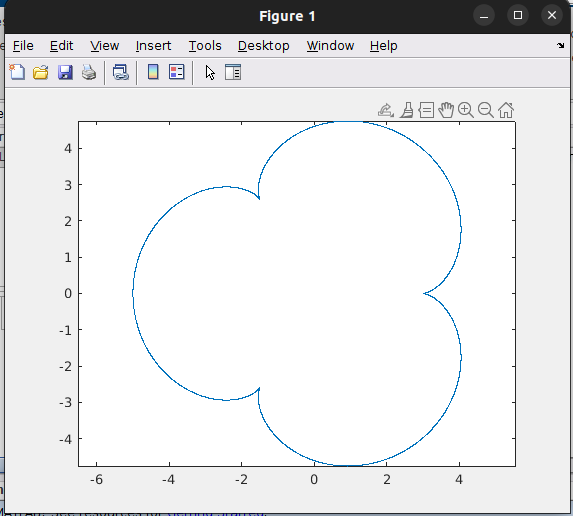
\includegraphics[width=0.5\linewidth]{./res1.png}
		\caption{结果:画出图}
	\end{figure}
	\item[3.] 画出轨迹图
	
	解: 因为椭圆参数曲线为$(a\cos(t), b\sin(t))$, 可知其标架为 
	\[e_1 = \dfrac{(-a\sin t, b \cos t)}{\sqrt{a^2 \cos^2t + b^2 \sin^2t}}, e_2 = \dfrac{(- b \cos t, -a\sin t)}{\sqrt{a^2 \cos^2t + b^2 \sin^2t}}.\]
	并且曲率是
	\[\kappa (t) =  \dfrac{ab}{(a^2\sin^2t + b^2 \cos^2 t)^{\frac{3}{2}}}.\]
	所以可以直接编程实现。
	\begin{figure}[hptb]
		\centering
		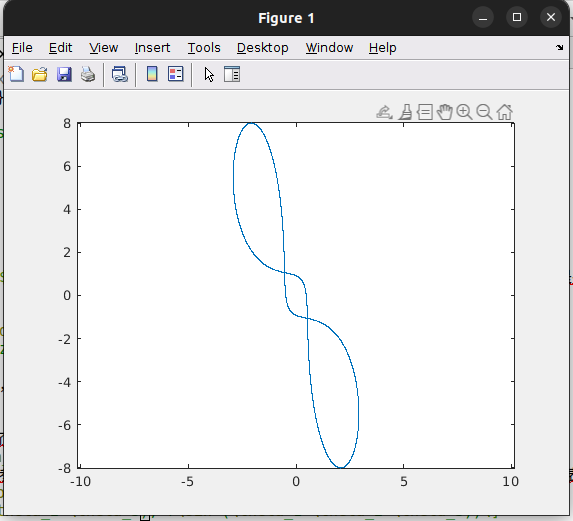
\includegraphics[width=0.5\linewidth]{./res2.png}
		\caption{当:$a = 2, b = 1$时的结果。}
	\end{figure}
\end{itemize}
	
\end{document}
